\subsection{Acesso pela jusante}
%TODO Abelha: prós e contras do acesso, soluções, apresentar soluções de
% logística


Como última opção de acesso ao rotor, existe a possibilidade de utilização do
tubo de sucção ou descarga como meio de entrada à turbina. Com o fluxo de água
parado, é possível utilizar o Rio como meio de lançamento do sistema. A
complexidade da operação para utilizar esse acesso é maior, entretanto existem
vantagens que podem tornar essa solução viável e mais atrativa.

\textbf{Vantagens}
\begin{itemize}
  \item Virtualmente nenhuma restrição de tamanho
  \item Flexibilidade de soluções
  \item Facilidade de utilização de um manipulador industrial padrão
  \item Possibilidade de implementação em outras usinas
\end{itemize}

\textbf{Desvantagens}
\begin{itemize}
  \item Complexidade de lançamento e recuperação
  \item Custo
  \item Possibilidade de correnteza
  \item Complexidade logística de transporte entre a entrada do tubo de sucção e
  o aro câmara
  \item Complexidade de prototipação
\end{itemize}

As soluções foram divididas em etapas necessárias para a operação, ou
seja, lançamento e recuperação do sistema, logística de transporte e o robô de
metalização propriamente dito.

Para esse acesso, o maior obstáculo presente é o desenvolvimento de um sistema
de lançamento e recuperação do robô, a partir do rio, até o interior da turbina.
Essa operação deverá ser realizada com a turbina alagada e, em seguida,
pode-se dar início ao processo de drenagem da
mesma.
É importante que o sistema de lançamento seja robusto e garanta o perfeito posicionamento do robô dentro da turbina, assim
como, a sua recuperação, uma vez que o sistema não pode se perder no leito do
rio.

Primeiramente, o sistema deve ser a prova d'água com classificação de pelo
menos 50m.
Sendo assim, um vaso de pressão para o transporte do robô até o interior da turbina deve ser
desenvolvido, não havendo necessidade do maniupulador responsável pela
metalização em si ser a prova d'água. O \textit{container} de transporte
submarino deve ser menor que o tamanho do vão do stoplog, uma vez que ele
utilizirá esse caminho para acessar o tubo de descarga. Por outro lado, suas
dimensões devem ter o tamanho mínimo para que o robô e todo o material
necessário seja transportado. Há a necessidade, também, de uma escotilha que
 de acesso de tamanho suficiente para que todo o sistema seja retirado do seu
 interior.

Para o sistema de lançamento foi deslumbrada uma estrutura de transporte que
utilizará o pórtico rolante e o trilho guia dos stoplogs. Após a submersão da
estrutura, um mecanismo de lançamento, inspirado em um paletizador, é
responsável pelo posicionamento do \textit{container} sempre no mesmo ponto em
relação ao tubo de descarga. Com o vaso de pressão posicionado, a turbina deve
ser, então, drenada. Em seguida, o robô pode ser retirado de seu
envólucro e a operação de metalização pode ter seu início. Uma etapa crítica da
operação é a recuperação do sistema, na qual a turbina deve ser novamente
alagada e os os stoplogs retirados. S estrutura de transporte deve, então,
recuperar o \textit{container} transportador na mesma posição em que o sistema
foi lançado. O sucesso dessa operação tem como \textbf{hipótese que a velocidade
de drenagem e a correnteza gerada por essa operação não são suficientes para
retirar o container (mais pesado que a água) de sua posição inicial}. 

A movimentação do robô do ponto de lançamento até o aro câmara deverá ser
realizada a partir da utilização de cordas, roldanas e talhas. Caso necessário,
pode ser desenvolvido um sistema de locomoção com trilhos e/ou rodas atuadas
para o posicionamento automático do robô.

O robô de metalização pode ter diversos fomatos, mas devido a possilidade de se
utilizar um manipulador industrial padrão, o projeto inicial consiste em uma
base de apoio e um manipulador com alcance para o processamento de uma face da
pá posicionado de frente para pá, ou um manipulador posicionado entre duas pás com
alcance de para processar as duas as faces das pás voltadas para ele.

\subsubsection{Dimensionamento da base}

Para manipuladores com longo alcance, as forças e torques envolvidos requerem
uma estrutura de fixação do robô de forma que o sistema como um todo não se
movimente e, no caso extremo, tombe. Normalmente, os manipuladores robóticos são
fixados no chão e as características da superfície e dos parafusos são
estipulados pelo fornecedor a partir dos valores máximos de torque e força que o
manipulador pode exerce em sua base. Para uma base apoiada no chão, dois
fatores influenciam capacidade de estabilização da estrutura: o raio da base e o seu
peso.

O raio da base $r_{b_f}$ é limitado pelo ambiente da turbina e para cada escolha
de posicionamento existem restrições específicas. 
Para a realização dos cálculos de dimensionamento foi considerado,
primeiramente, o manipulador posicionado em frente a pá e processando somente uma face por vez
e a uma altura de 1000mm, posição em que o alcance necessário do robô é de
1800mm. Para essas características, a dimensão máxima perpendicular ao fluxo d'água que a base 
pode assumir é de aproximadamente 1600mm, caso a estrutura seja
 projetada de forma a seguir os contornos do aro câmara.
A figura \ref{fig::base_aro_frente} 
representa um esboço da vista frontal do aro câmara e a largura máxima que a
base pode assumir. A análise da dimensão máxima da base no sentido paralelo ao
fluxo d'água pode ser realizada com o auxílio do desenho técnico fornecido pela
ESBR, ilustrado na figura \ref{fig::turbine_side}. 
%TODO Gabriel-Renan -pedir pro renan a figura da camara
O limite superior nessa
região é determinado pela transição do aro câmara para a região inclinada do
tubo de sucção e é de aproximadamente 1600mm. Entrentanto esse limite pode ser
contornado construindo-se um plano horizontal ou projetando-se a base de forma que ela acompanhe essa
inclinação. Ao se incluir o dimensionamento da base no cálculo do alcance mínimo
do manipulador deve ser realizado uma alteraçao, uma vez que agora o manipulador
se encontra deslocado da superfície da pá. Sendo assim, alcance mínimo se
relaciona com o tamanho do raio da base de acordo com
$$a_{min}=\sqrt{r_b^2+1800^2}.$$

\begin{figure}[h!]
\centering
	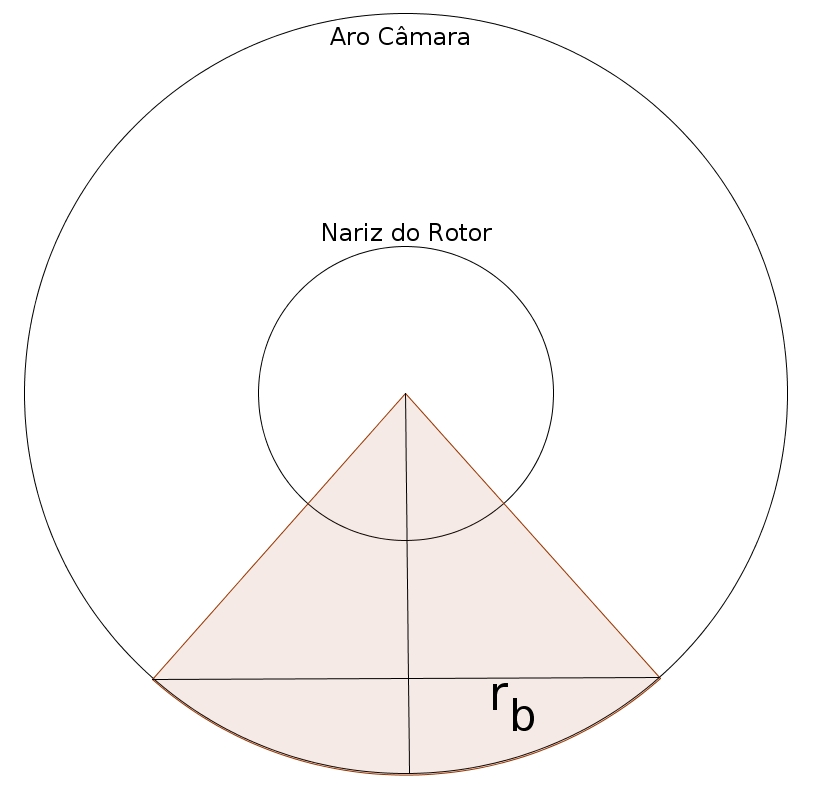
\includegraphics[width=0.9\columnwidth]{figs/base/base_aro_frente.jpg}
	\caption{Visão frontal do aro câmara e raio máximo da base.}
	\label{fig::base_aro_frente}
\end{figure}

O cálculo das dimensões da base com o robô posicionado dentro do aro câmara e
entre as pás depende do angulo de ataque das pás e do cálculo do ângulo diédrico
entre elas de acordo com o seu ângulo de ataque. A amplitude do movimento de
rotação $alpha$ das pás é de $14,5^o$ para cada lado a partir da posição zero, entretanto \textbf{essa posição não pôde ser
informada no momento da viagem de reconhecimento e ainda não foi
disponibilizada}. Para critério de cálculos foi utilizado um ângulo de
$45^o$ como a posição de maior abertura das pás e o zero foi considerado como
a reta perpendicular ao fluxo de água. O ângulo diédrico $\theta$ entre as pás depende da rotação
sofrida pelas mesmas e obedece a relação $\cos{\theta} = \sin^2{\alpha}.$

O arco de circunferência pode ser obtido a partir da relação $arc=R\alpha$, com
R=3850mm. O raio máximo da base pode ser calculado como 
$$r_{b_e} = (R - h_{b_e})\tan{\theta/2},$$  ilustrado na figura
\ref{fig:calc_base_entre} e com $h_{b_e}$ sendo a altura da base.

O peso mínimo que a base do robô deve possuir está diretamente relacionada com o
tamanho de seu raio. A firgura \ref{fig::tilt_robot} faz uma representação
simplificada da forma que o torque de capotamento máximo atua no robô e em sua
base. Na situação limite, considerando o torque com sentido horário, a força
normal entre a base e a superfície de apoio $N_2$ teria módulo igual a zero.
Considerando o pior caso, ou seja, a força vertical que o robô exerce na base é
composta apenas pelo seu peso $W$ para que a base não se mova durante a
operação, temos que o somatório das forças e torques sejam iguais a zero.

A análise das forças nos fornece que $N_1$ tenha módulo igual ao peso do robô e
o somatório dos torques se reduz a $M_k-Wr_b=0$. Sendo assim, a relação entre
o raio da base, seu peso e o torque máximo de capotamento exercido pelo robô é
da forma 

$$M_k=Wr_b.$$

%TODO refazer figura
\begin{figure}[h!]
\centering
	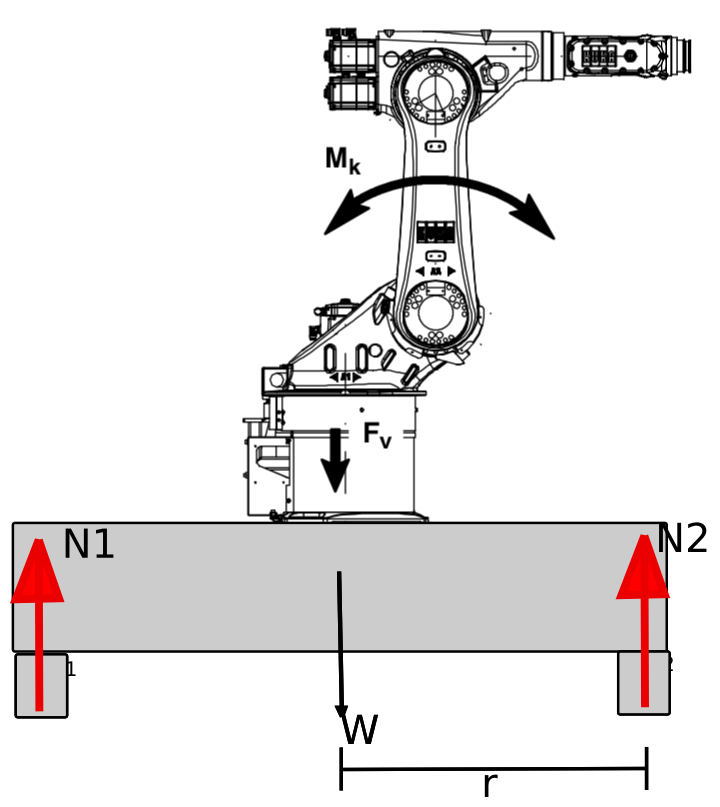
\includegraphics[width=0.5\columnwidth]{figs/base/tilt}
	\caption{Forças e torques máximos entre o robô e sua base.}
	\label{fig::tilt_robot}
\end{figure}

Uma vez que a superfície do aro câmara e a região adjacente no tubo de sucção
são \textbf{ferromagnéticas}, é possível a utilização de bases magnéticas para
uma compensação do peso e raio necessários para a estabilização do robô. Os
dispositivos magnéticos se dispõem de duas em duas principais catergorias para
essa aplicação:
dispositivos eletretromagnéticos e de imãs permanentes. O primeiro caso tem como
principal vantagem a possibilidade de acionamento remoto, entretanto para situações de
falha em que haja perda de fornecimento de energia, a força de atração também é
perdida. O segundo caso consiste em imãs permanentes arrumados de maneira que
seja possível organizar o seu fluxo magnético e, assim, controlar por meio de
uma alavanca a presença ou ausência de força magnética. A figura
\ref{fig::base::imas} ilustra os dois tipos de bases magnéticas citados.

\begin{figure}[h!]
\begin{subfigure}[b]{0.5\columnwidth}
  \centering
  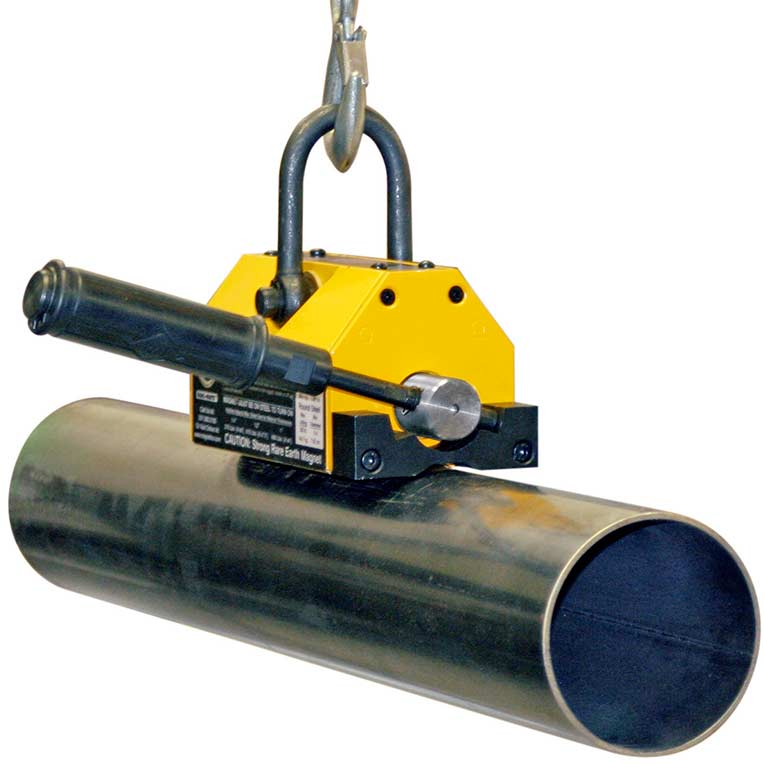
\includegraphics[width=.9\columnwidth]{figs/base/mangnetpipe}
  \caption{Tipo imã permanente}
  \label{fig:sfig1}
\end{subfigure}%
\begin{subfigure}[b]{0.4\columnwidth}
  \centering
  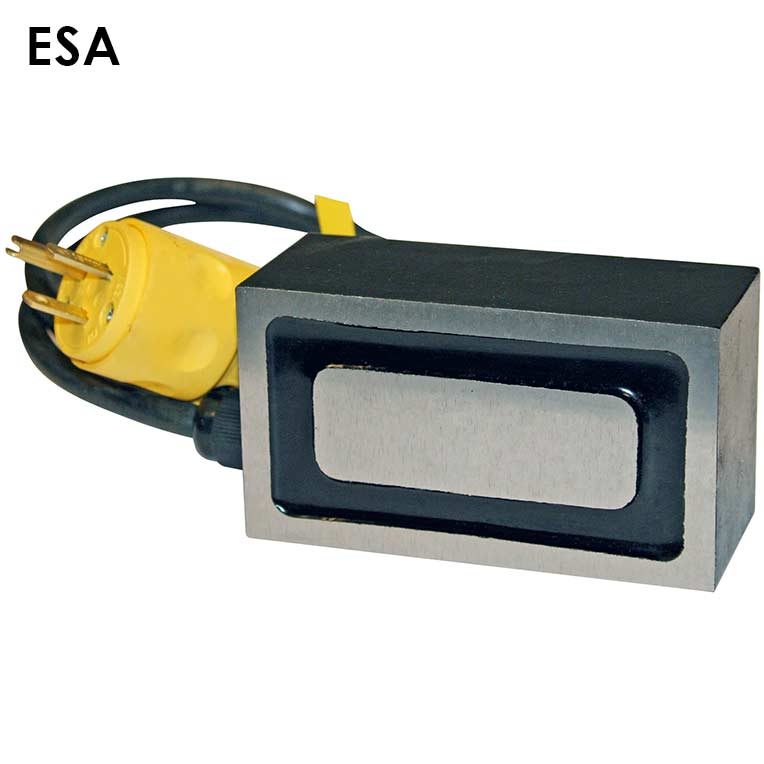
\includegraphics[width=.9\columnwidth]{figs/base/eletromagnet}
  \caption{Tipo eletroimã}
  \label{fig:sfig2}
\end{subfigure}
\caption{Tipos de bases magnéticas comerciais.}
\label{fig::base::imas}
\end{figure}

Comercialmente, foram encontrados bases magnéticas com capacidade de até 3000N.
Um dos requerimentos para a utilização de bases magnéticas, sejam
eletromagnéticas e de imãs permanentes, é a limpeza da superfície de contato
para um acoplamento efeiciente. Essa restrição força a presença humana para a
limpeza e, sobretudo, a verificação de uma correta fixação. Sendo assim, as
bases magnéticas de imã permanente se mostram mais coerentes para a aplicação,
pois não possuem ponto de falha para o caso de perda de energia do sistema e
possuem uma maior capacidade de carga. A curvatura do ambiente não é um
limitante, sendo possível até a confecção de uma máscara para a base de maneira
que a superfície de apoio se conforme perfeitamente com a superfície de fixação.












